Nu doen we hetzelfde, maar in plaats van equidistante abscissen gebruiken we nu Chebyshev-punten. Het  resultaat voor $sin(x)$ is te vinden in figuur \ref{fig:sincheb}, het resultaat voor $\frac{1}{1+7x^2}$ in figuur \ref{fig:ratcheb}. We geven ook hier steeds een plot van de functiewaarden en van het residu weer.
\\
Het gebruik van Chebyshev-punten is een duidelijke verbetering, vooral aan de rand van het interval. 
\\
TODO verdere uitleg over verschil veelterm vs. spline

\begin{figure}
\centering
\begin{subfigure}{.5\textwidth}
  \centering
  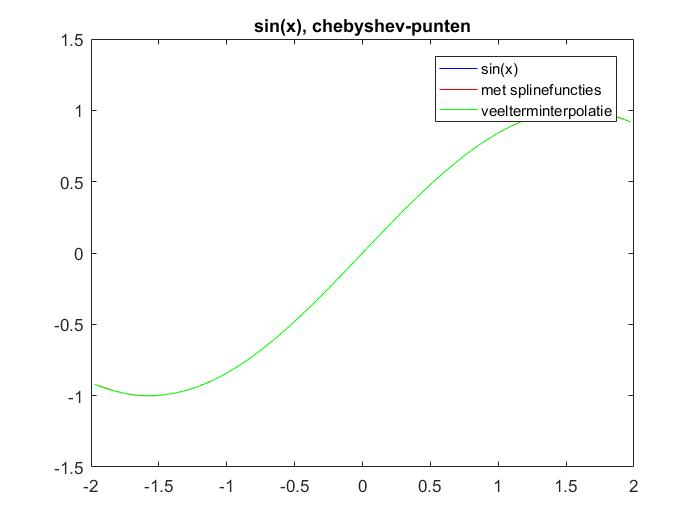
\includegraphics[width=\linewidth]{afbeeldingen/sin_cheb.jpg}
  \caption{functiewaarden}
\end{subfigure}%
\begin{subfigure}{.5\textwidth}
  \centering
  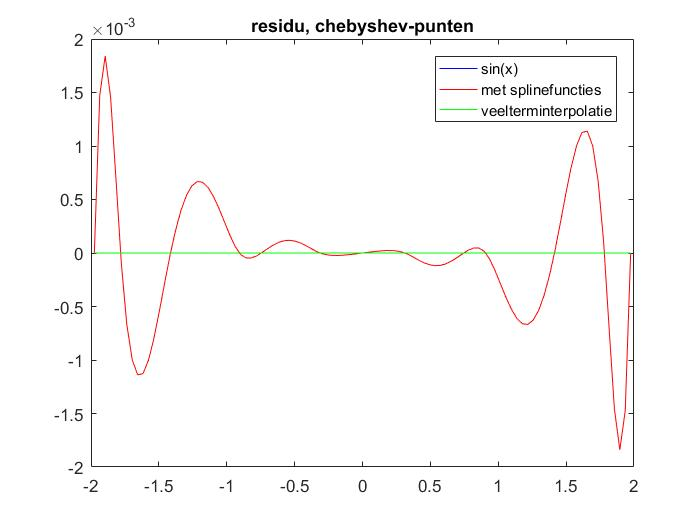
\includegraphics[width=\linewidth]{afbeeldingen/sin_cheb_res.jpg}
  \caption{residu}
\end{subfigure}
\caption{interpolant door 10 Chebyshev-punten van $sin(x)$}
\label{fig:sincheb}
\end{figure}

\begin{figure}
\centering
\begin{subfigure}{.5\textwidth}
  \centering
  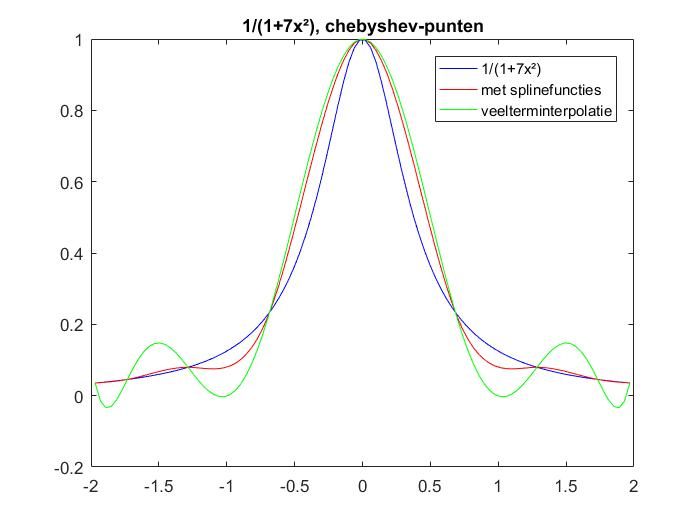
\includegraphics[width=\linewidth]{afbeeldingen/rat_cheb.jpg}
  \caption{functiewaarden}
\end{subfigure}%
\begin{subfigure}{.5\textwidth}
  \centering
  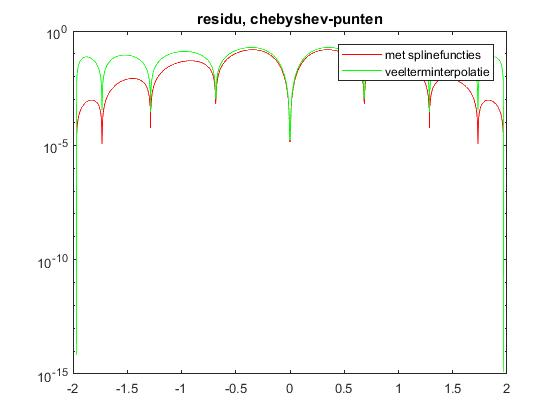
\includegraphics[width=\linewidth]{afbeeldingen/rat_cheb_res.jpg}
  \caption{residu}
\end{subfigure}
\caption{interpolant door 9 Chebychev-punten van  $\frac{1}{1+7x^2}$}
\label{fig:ratcheb}
\end{figure}